\chapter{トレースログ可視化ツール TraceLogVisualizer の利用}

\section{トレースログの可視化}
本節では,開発したTLVを用いて,様々な形式のトレースログの可視化を行い,汎用性があることを確認する.

まず,シングルコアプロセッサ用RTOSの可視化を行い,動作の確認を行う.
次に,マルチコアプロセッサ用RTOSの可視化に対応するように拡張し,どの程度の作業で拡張が行えるのかを確認する.
最後に,組込みコンポーネントシステムの可視化を行い汎用性の確認を行う.

\subsection{シングルコアプロセッサ用RTOSのトレースログの可視化}
可視化するシングルコアプロセッサ用RTOSとして,TOPPERS/ASPカーネルを用いた.TOPPERS/ASPカーネルは,標準でトレースログを取得する機能を搭載しており,カーネルの動作開始と終了,処理単位の実行開始と終了,タスク状態の変化,ディスパッチャの実行開始と終了,サービスコールの入口と出口といった情報をトレースログ取得できる.
処理単位とは,割込みハンドラ,割込みサービスルーチン,周期ハンドラ,アラームハンドラ,CPU例外ハンドラ,タスク例外処理ルーチンを指す.

可視化表示する項目は,タスクの状態遷移,システムコール,実行タスクの遷移とした.

タスクの状態遷移の可視化表現は,実行状態を緑色の四角形,実行可能状態を黄色い線分,待ち状態を赤い線,休止状態を灰色の線,起動を上矢印,終了を下矢印とする.
図\ref{fig:taskStateChangeVisual}にタスクの状態遷移の可視化表現の例を示す.

システムコールの可視化表現は,赤色の四角形で,枠線を点線,高さを待ち状態の線と同じ高さとする.
このとき,システムコール名,システムコールの引数を四角形の上左隅,返値であるエラーコードを下右隅に文字列で出力するとする.
図\ref{fig:svcCallVisual}にシステムコールの可視化表現の例を示す.

実行タスクの遷移の可視化表現は,四角形で,上左隅に実行タスク名を文字列を出力するとする.
また,四角形の色を実行タスク毎に変えて出力するとする.
図\ref{fig:runningTaskChangeVisual}に実行タスクの遷移の可視化表現の例を示す.

\begin{figure}[t]
\begin{center}
\includegraphics[scale=0.75]{img/taskStateChangeVisual.eps}
\caption{タスクの状態遷移の可視化表現例}
\label{fig:taskStateChangeVisual}
\end{center}
\begin{tabular}{cc}
\begin{minipage}{0.5\hsize}
\begin{center}
\includegraphics[height=3cm]{img/svcCallVisual.eps}
\caption{システムコールの可視化表現例}
\label{fig:svcCallVisual}
\end{center}
\end{minipage}
\begin{minipage}{0.5\hsize}
\begin{center}
\includegraphics[height=3cm]{img/runningTaskChangeVisual.eps}
\caption{実行タスクの遷移の可視化表現例}
\label{fig:runningTaskChangeVisual}
\end{center}
\end{minipage}
\end{tabular}
\end{figure}






\subsection{マルチコアプロセッサ用RTOS対応への拡張}

\subsection{組み込みコンポーネントシステムの可視化}

\section{可視化表示項目の追加・変更}
